\chapter{DCM for Induced Responses \label{Chap:data:dcm_ir}}

This chapter shows an example of Dynamic Causal Modelling for Induced Responses (DCM-IR) \cite{cc_induced}. The example is based on the analysis described by Chen et al. \cite{cc_asymm}. The purpose of the analysis is to look at the effective connectivity between cortical areas involved in the processing of faces and specifically at non-linearities in the connections expressed as cross-frequency coupling. DCM-IR is an example of a phenomenological rather than physiological DCM. The advantage of this approach is that it can directly model a particular feature extracted from the data, namely event-related spectral perturbations. This feature has been a popular object of study in the neuroscience literature. However, since computing event-related power involves discarding phase information, it is not possible to model this feaure with a physiologically realistic model such as the one used in DCM for evoked responses. An important feature of DCM for induced responses is that it models the full time-frequency spectrum. This differs from typical approaches, where a few specific frequency bands are selected \textit{a priori}. DCM-IR models spectral dynamics in terms of a mixture of frequency modes (obtained with singular value decomposition). The dynamics of each mode are encoded by the evolution of a state. It is this multi-state vector, for each source, that captures how the energy in different frequencies interacts, either linearly or non-linearly, among sources.

\section{Data}

We will use the epoched and merged MEG dataset from Chapter~\ref{multimodal:data:meg} saved in the files:

\begin{verbatim}
cdbespm8_SPM_CTF_MEG_example_faces1_3D.mat
cdbespm8_SPM_CTF_MEG_example_faces1_3D.dat
\end{verbatim}

See ~\ref{multimodal:data:meg:preproc} for the instructions for how to generate these files from raw MEG data. DCM-IR also requires a head model and coregistration. If you have performed ``Imaging'' reconstruction of differential power \ref{multimodal:data:meg:recon_pow} and saved the results, the head model should already be defined. Otherwise, you will be asked to define the head model while configuring the DCM (see below).

\section{Getting Started}

You need to start SPM and toggle ``EEG'' as the modality (bottom-right of SPM main window), or start SPM with \texttt{spm eeg}. In order for this to work you need to ensure that the main SPM directory is on your \matlab\ path.

\section{Setting up DCM}

After calling \texttt{spm eeg}, you see SPM's graphical user interface, the top-left window. The button for calling the DCM-GUI is found in the second partition from the top, on the right hand side. When pressing the button, the GUI pops up (Figure~\ref{dcm-ir:fig:1}). The GUI is partitioned into five parts, going from the top to the bottom. The first part is about loading and saving existing DCMs, and selecting the type of model. The second part is about selecting data, the third is for specification of the spatial forward model, the fourth is for specifying connectivity, and the last row of buttons allows you to estimate parameters and view results.

\begin{figure}
\begin{center}
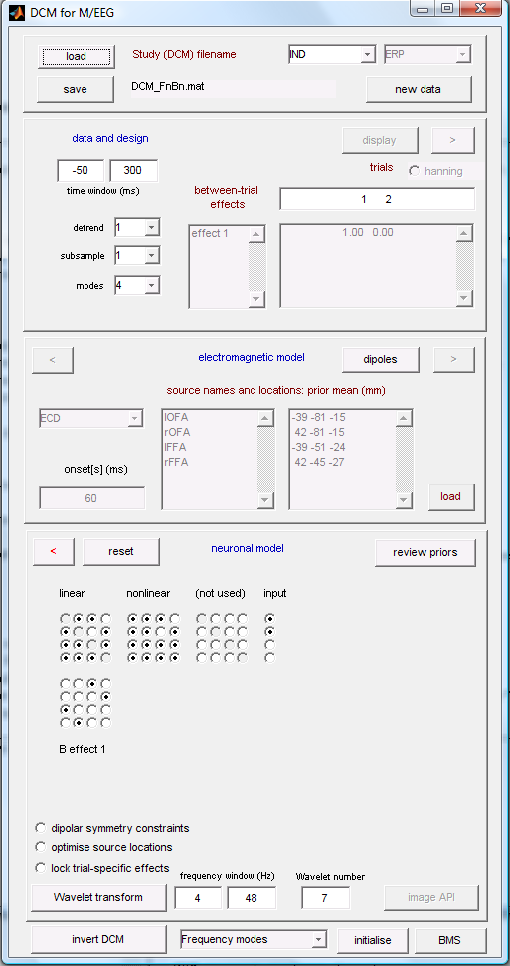
\includegraphics[width=100mm]{dcm_ir/figures/irfigure1}
\caption{\em DCM window configured analysing induced responses and the FnBn model specified.\label{dcm-ir:fig:1}}
\end{center}
\end{figure}

You have to select the data first and specify the model in a fixed order (data selection $>$ spatial model $>$
connectivity model). This order is necessary, because there are dependencies among the three parts that would be hard to resolve
if the input could be entered in any order. At any time, you can switch back and forth from one part to the next. Also, within each part, you can specify information in any order you like.

\subsection{load, save, select model type}
At the top of the GUI, you can load an existing DCM or save the one you are currently working on. In general, you can \texttt{save} and \texttt{load} during model specification at any time. You can also switch between different DCM analyses (the left menu). The default is ``ERP'' which is DCM for evoked responses. You should switch to ``IND'' which is the option for DCM-IR. The menu on the right-hand side lets you choose the neuronal model. Once you switch to ``IND'', it will be disabled since neuronal models are not relevant for DCM-IR, which is a phenomenological DCM.

\subsection{Data and design}
In this part, you select the data and model between-trial effects. Press ``new data'' and select the data file \texttt{cdbespm8\_\-SPM\_\-CTF\_\-MEG\_\-example\_\-faces1\_\-3D.mat}.The data file will usually be an epoched file with multiple trials per condition. These data must be in SPM-format. On the right-hand side you can enter trial indices of the evoked responses in this SPM-file. For example, if you want to model the first and second condition contained within an SPM-file, specify
indices \texttt{1} and \texttt{2}. You can type:
\begin{verbatim}
D = spm_eeg_load(`cdbespm8_SPM_CTF_MEG_example_faces1_3D.mat');D.condlist
\end{verbatim}
in the command line to see the list of condition labels in the order that corresponds to these indices. This order is defined in the dataset and can be modified by selecting ``Sort Conditions'' from the ``Other'' submenu in main SPM window (\textit{spm\_eeg\_sort\_conditions}). SPM should echo:
\begin{verbatim}
ans = 

    'faces'    'scrambled'
\end{verbatim}
meaning that index \texttt{1} corresponds to presentation of faces and index \texttt{2} - to presentation of scrambled faces. The box below the list of indices allows specifying experimental effects on connectivity. The specification can be quite generic as in the design matrix for a General Linear Model (GLM). Our case is quite simple though. We have a baseline condition which is ``scrambled'' and we would like to know how the condition of interest ``faces'' differs from it. We will therefore enter:
\begin{verbatim}
1 0
\end{verbatim}
in first row of the box, which means that there will be some additive modulation of connections that we will define later for ``faces''  (some coefficient multiplied by 1) and this modulation will not be there for ``scrambled'' (the same coefficient multiplied by 0). If we now click somewhere outside the box, a default name will be assigned to this effect - ``effect1''. It will appear in the small text box next to the coefficients box. It is possible to change this name to something else e.g. ``face''.

Now we can select the peristimulus time window we want to model. These are the two test boxes in the top left corner of the panel. Enter \texttt{-50} in the left box and \texttt{300} in the right box to select the segment \texttt{-50} to \texttt{300} ms relative to the presentation of the visual stimulus.  

You can choose whether you want to remove low-frequency drifts of the data at sensor level. If you don't, select \texttt{1} for ``detrend'', to just remove the mean. Otherwise select the number of discrete cosine transform terms you want to remove. You can also subsample your data (prior to computing the time-frequency decomposition) using the ``subsample'' option. In general, it is advised to filter out drifts and downsample the data during preprocessing. The options here are just to \textit{play around} with, clean up or reduce the data to see what effect it might have without running additional processing steps outside DCM.

Press the ``Display'' button to look at the selected data. You will see the evoked responses for the two conditions (Figure~\ref{dcm-ir:fig:2}) which help you get some idea about your choice of time window. It is possible to change the ``detrend'' and ``subsample'' values or the time window and press ``Display' again to see what effect these changes have. 

An important parameter for DCM-IR is the number of modes. These are the frequency modes mentioned above. The idea is that the main features of the time-frequency image can be represented by a small number of components with fixed frequency profiles that are modulated over time. These components can be determined automatically using ``Singular Value Decomposition'' (SVD). Generally SVD preserves information from the original time-frequency image and produces as many components as there are frequency bins. However, usually only the first few components are physiologically relevant and the rest are just noise. Using a small number of components will greatly speed-up DCM model inversion. You cannot know in advance what the optimal number of components for your data is. What you can do is try once with a relatively large number (e.g. 8) and then see from the time and frequency profile of the later components (in the Results view, see below) whether they are important. Then you can reduce the number and try again. For the example here it is sufficient to use 4 modes so change the number in ``modes'' from 8 to 4. 

\begin{figure}
\begin{center}
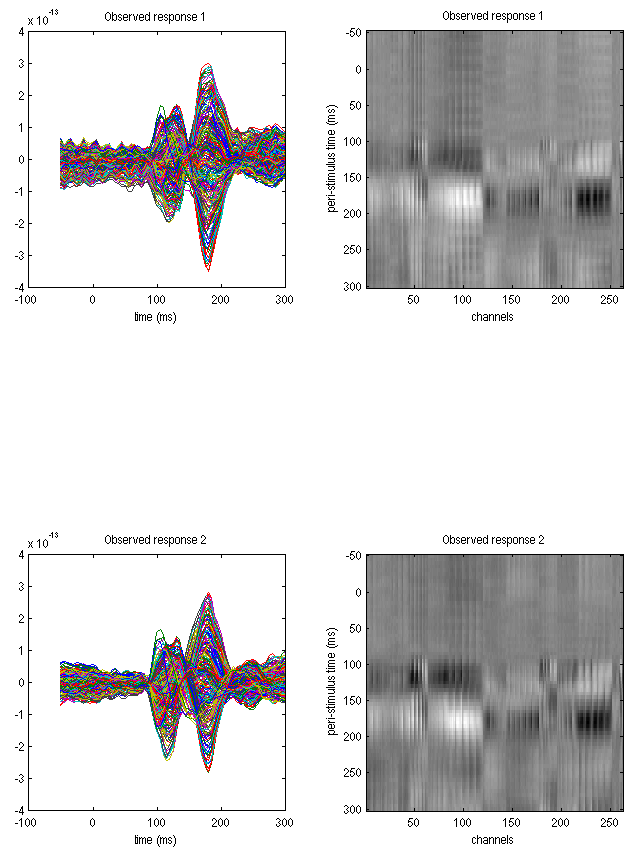
\includegraphics[width=160mm]{dcm_ir/figures/irfigure2}
\caption{\em Averaged evoked responses after configuring the 'Data and design' section.\label{dcm-ir:fig:2}}
\end{center}
\end{figure}

If you are happy with your data selection, the subsampling and the detrending terms, you can click on the $>$ (forward) button, which will bring you to the next stage \textit{electromagnetic model}. From this part, you can press the red $<$ button to get back to the data and design part.

\subsection{Electromagnetic model}
With DCM-IR, you have two options for how to extract the source data for time-frequency analysis. Firstly, you can use 3 orthogonal single equivalent current dipoles (ECD) for each source and invert the resulting source model to get source waveforms. This option is suitable for multichannel EEG or MEG data. Alternatively, you can treat each channel as a source (LFP option). This is appropriate when the channels already contain source data either recorded directly with intracranial electrodes or extracted (e.g. using a beamformer). 

Note that a difference with DCM for evoked responses is that the parameters of the spatial model are not optimized. This means that DCM-IR will project the data into source space using the spatial locations you provide.

We will use the ECD option. This requires specifying a list of source names in the left large text box and a list of MNI coordinates for the sources in the right large text box. Enter the following in the left box:

\begin{verbatim}
lOFA
rOFA
lFFA
rFFA
\end{verbatim}

Now enter in the right text box:

\begin{verbatim}
-39 -81 -15
 42 -81 -15
-39 -51 -24
 42 -45 -27
\end{verbatim}

These correspond to left Occipital Face Area, right Occipital Face Area, left Fusiform Face Area and right Fusiform Face Area respectively. See \cite{cc_induced} for more details.

The onset-parameter determines when the stimulus, presented at 0 ms peri-stimulus time, is assumed to trigger the cortical induced response. In DCM, we usually do not model the rather small early responses, but start modelling at the first large deflection. Because the propagation of the stimulus impulse through the input nodes causes a delay, we found that the default value of 60
ms onset time is a good value for many responses where the first large deflection is seen around 100 ms. However, this value is a
prior, i.e. the inversion routine can adjust it. The prior mean should be chosen according to the specific responses of interest. This is because the time until the first large deflection is dependent on the paradigm or the modality you are working in, e.g. audition or vision. You may also find that changing the onset prior has an effect on how your data are
fitted. This is because the onset time has strongly nonlinear effects (a delay) on the data, which might cause differences in the maximum found at convergence, for different prior values. Note, that it is possible to enter more than one number in the ``onset[s] (ms)'' box. This will add several inputs to the model. These inputs can then be connected to different nodes and/or their timing and frequency profiles can be optimized separately.

When you want to proceed to the next model specification stage, hit the $>$ (forward) button and proceed to the \textit{neuronal model}. If you have not used the input dataset for 3D source reconstruction before you will be asked to specify the parameters of the head model at this stage. See ~\ref{multimodal:data:meg:recon_pow}.

\section{Neuronal model}
There are 4 (or more) matrices which you need to specify by button presses. In the first row there are matrices that define the connectivity structure of the model and in the second row there are matrices that specify which connections are affected by experimental effects. All the matrices except one are square. In each of these square matrices you specify a connection \textit{from} a source area \textit{to} a target area. For example, switching on the element $(2,\;1)$ means that you specify a connection from area 1 to 2 (in our case from lOFA to rOFA). Some people find the meaning of each element slightly counter-intuitive, because the column index corresponds to the source area, and the row index to the target area. This convention is motivated by direct correspondence between the matrices of buttons in the GUI and connectivity matrices in DCM equations and should be clear to anyone familiar with matrix multiplication.

The leftmost matrix in the first row specifies the \textit{linear} connections. These are the connections where frequency dynamics in one source affects the dynamics at the same frequencies in another source. Note that all connections in the model should be at least linear, so if you think some connection should be present in the model, the corresponding button in this matrix should be on. Also the buttons on the leading diagonal of the matrix are always on because each node in the model has a linear  intrinsic connection with negative sign. This means that the activity has a tendency to dissipate. To the right of the linear connectivity matrix there is a \textit{nonlinear} connectivity matrix. The idea here is the same, just remember to enable the corresponding linear connection as well. When a connection is nonlinear, a frequency mode in the source node can affect all the frequency modes in the target node. Intrinsic connections can be made non-linear as well. It is actually recommended to always make the intrinsic connections non-linear unless there is a good theoretical reason not to do it. Since we are mainly interested in non-linearities in the extrinsic connections we would like to be over-conservative and first explain away anything that can be explained by non-linearities in the intrinsic connnections.

The rightmost matrix in the first row is the input matrix. It is usually not square, and in the case of a single input, as we have here, is reduced to a column vector. The entries of this vector specify which areas receive the external input (whose onset time we specified above). In the case of several inputs the input matrix will have several columns.

The matrix (matrices) in the second row specify which of the connections defined in the first row can be modified by experimental effects. A connection which is not modified will have the same value for all conditions. If you don't allow modification of any of the connections, then exactly the same model will be fitted to all conditions. For the purpose of allowing modification by experimental effects, it does not matter whether a connection is linear or non-linear. Hence, there is one modulation matrix per experimental effect (defined in the ``Data and design'' panel). In our case there is only one effect - faces vs. scrambled faces. Also self connections can be modified by experimental effects, thus the diagonal entries of the second row matrices can also be toggled.

Figure ~\ref{dcm-ir:fig:3} is taken from the paper of Chen et al. \cite{cc_asymm} and shows several alternative models that could apply to the data. We will start by specifying the model with nonlinear forward and backward connections (FnBn) and with effect of condition on these connections. The corresponding button configuration is shown in Figure ~\ref{dcm-ir:fig:4}. Compare the depiction of FnBn model in Figure~\ref{dcm-ir:fig:3}  with the specification in Figure~\ref{dcm-ir:fig:4}  to see the correspondence. Note that the effect of condition is not shown in Figure~\ref{dcm-ir:fig:3}. Now copy the specification to the DCM GUI.

\begin{figure}
\begin{center}
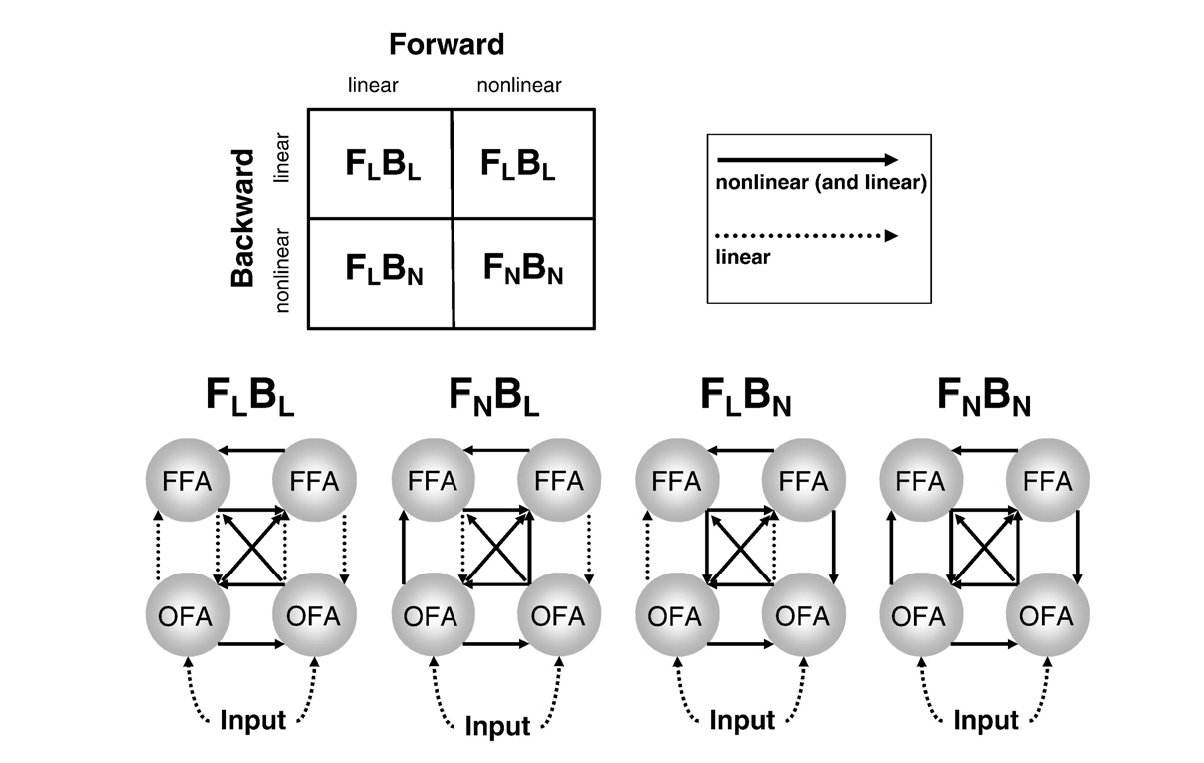
\includegraphics[width=160mm]{dcm_ir/figures/irfigure3}
\caption{\em Four different DCM-IR models proposed by Chen et al. \cite{cc_asymm} \label{dcm-ir:fig:3}}
\end{center}
\end{figure}

\begin{figure}
\begin{center}
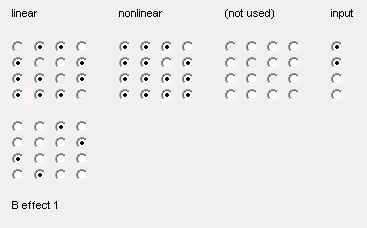
\includegraphics[width=60mm]{dcm_ir/figures/irfigure4}
\caption{\em Connectivity configuration for the FnBn model.\label{dcm-ir:fig:4}}
\end{center}
\end{figure}

At the bottom of this panel there are additional radio buttons for options that are not relevant for DCM-IR. Below these buttons there are controls for specifying the parameters of the wavelet transform for computing the time-frequency decomposition. We will keep the default frequency window 4 to 48 Hz and increase the number of wavelet cycles to 7. You can press the \textit{Wavelet transform} button to preview the time-frequency plots and optimize the parameters if necessary before inverting the model.  


\section{Estimation}
When you have finished model specification, you can hit the \textit{invert DCM} button in the lower left corner. DCM will now estimate the model parameters. You can follow the estimation process by observing the model fit in the output window. Note that in DCM-IR there is no difference between the hidden states and the predicted responses because the dynamics of the hidden states fit directly the time course of frequency modes (shown as dotted lines in the middle plot). This is different from DCM for ERP where the hidden states correspond to neural dynamics and a subset of the hidden states (activation of pyramidal cells) are projected via the forward model to generate predictions of sensor data. In the \matlab\ command window, you will see each iteration print an expectation-maximization iteration number, free energy $F$, and the predicted and actual change of $F$ following each iteration step. At convergence, DCM saves the results in a DCM file, by default named \texttt{DCM\_*.mat} where \texttt{*} corresponds to the name of the original SPM MEG file you specified. You can save to a different name, e.g. if you are estimating multiple models, by pressing 'save' at the top of the GUI and writing to a different name.

\section{Results}
After estimation is finished, you can assess the results by choosing from the pull-down menu at the bottom (middle).

\subsection{Frequency modes}
This will display the frequency profiles of the modes, identified using singular value decomposition of spectral dynamics in source space (over time and sources).

\subsection{Time modes}
This will display the observed time courses of the frequency modes (dashed lines) and the model predictions (solid lines). Here you can also see whether the activity picked up by the minor modes is noise, which is helpful for optimizing the number of modes. 

\subsection{Time-Frequency}
This will display the observed time-frequency power data for all pre-specified sources (upper panel) and the fitted data features (lower panel).

\subsection{Coupling (A-Hz)}
This will display the coupling matrices representing the coupling strength from source to target frequencies. These matrices are obtained by multiplying the between-mode matrices estimated with the frequency profiles of the modes (see \cite{cc_induced}). The arrangement of the matrices corresponds to arrangements of the buttons in the connectivity matrices above.

\subsection{Coupling (B-Hz)}
This presentation of results is similar to the above and reports modification of coupling by condition (eg. in our example it shows which frequency couplings are different for faces as opposed to scrambled faces). 

\subsection{Coupling (A-modes)}
This will display the coupling matrices between modes and the conditional probabilities that the coefficients are different from zero. This representation is useful for diagnostics when something is wrong with the inversion, but the physiological interpretation is less straightforward.

\subsection{Coupling (B-Hz)}
This presentation is similar to the above and reports the modification of coupling by condition. 

\subsection{Input (C-Hz)}
This shows the frequency profiles of the inputs estimated. This is again a multiplication between the mode-specific coefficients and the frequency profiles of the modes. 

\subsection{Input (u-ms)}
This shows the time courses of the inputs.

\subsection{Dipoles}
This shows the positions of the sources as specified in the ``Electromagnetic model'' section.

\subsection{Save as img}
Here you can save the cross-frequency coupling matrices as images. If you are analyzing a group of subjects you can then enter these images into parametric statistical tests to find common features in coupling and coupling changes accross subjects. The image names will include identifiers like ``A12'' or ``B31'' which relate to the source connection matrices; either the basic (A) or experimental effects (B).

\section{Model comparison}

You can now compare the fully nonlinear model with alternative models (eg. those shown in Figure~\ref{dcm-ir:fig:3}). You can start by saving the DCM you have already specified under a different name using the \textit{Save} button. Then just modify the connectivity matrices and reinvert the DCM by pressing the ``Estimated'' button (but not using previous posterior or prior estimates). As an exercise, you can specify the other models from Figure~\ref{dcm-ir:fig:3} yourself. If in doubt look at Figure~\ref{dcm-ir:fig:5} for the three alternative models. Once you have specified and inverted the three additional models, you can perform Bayesian model comparison. 

\begin{figure}
\begin{center}
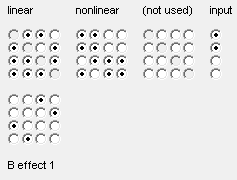
\includegraphics[width=40mm]{dcm_ir/figures/irfigure5_FlBl}
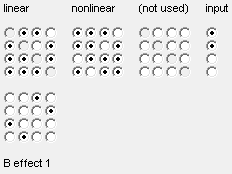
\includegraphics[width=40mm]{dcm_ir/figures/irfigure5_FlBn}
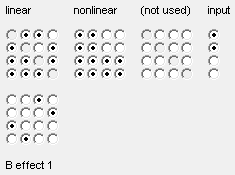
\includegraphics[width=40mm]{dcm_ir/figures/irfigure5_FnBl}
\caption{\em Connectivity configurations for the alternative models. Left to right: FlBl, FlBn, FnBl. \label{dcm-ir:fig:5}}
\end{center}
\end{figure}

Press the \textsc{BMS} button. This will open the SPM batch tool for model selection. Specify a directory to write the output file to.  For the ``Inference method'' select ``Fixed effects'' (see \cite{klaas_bms} for additional explanations). Then click on ``Data'' and in the box below click on ``New: Subject''. Click on ``Subject'' and in the box below on ``New: Session''. Click on models and in the selection window that comes up select the DCM mat files for all the models (remember the order in which you select the files as this is necessary for interpreting the results). Then run the model comparison by pressing the green ``Run'' button. You will see, at the top, a bar plot of the log-model evidences for all models ~\ref{dcm-ir:fig:6}. At the bottom, you will see the posterior probability, for each model, given the data. By convention, a model can be said to be the best among a selection of other models, with strong evidence, if its log-model evidence exceeds all other log-model evidences by at least 3. In our case the FnBn model is superior to the other models as was found in the original paper \cite{cc_asymm} for a different group of subjects. 

\begin{figure}
\begin{center}
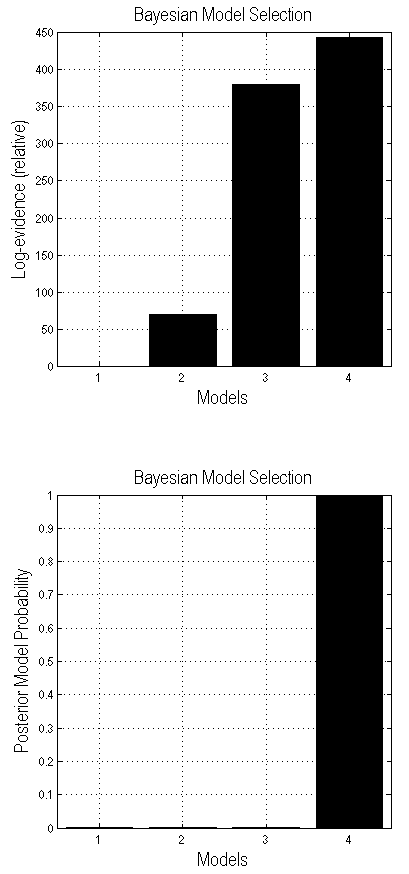
\includegraphics[width=50mm]{dcm_ir/figures/irfigure6}
\caption{\em Bayesian comparison of the four DCM-IR models shown in Figure~\ref{dcm-ir:fig:3}.\label{dcm-ir:fig:6}}
\end{center}
\end{figure}
